\section{Hipótese de Trabalho}

A hipótese deste estudo é: Ao integrar os resultados do LibScout aos contextos das ferramentas CryptoGuard e CogniCrypt, será possível não apenas detectar potenciais vulnerabilidades em APIs criptográficas, mas também identificar as correspondências associadas a bibliotecas externas. Esta integração proporciona uma abordagem mais abrangente e eficaz para a segurança de aplicações Java que utilizam operações criptográficas.

\section{Metodologia}

\subsection{Estrutura da Metodologia (GQM)}

Conforme discutido no Capítulo 1, os objetivos desta pesquisa incluem a identificação e análise de vulnerabilidades em APIs criptográficas Java, com foco na integração dos resultados obtidos pelo LibScout aos contextos fornecidos pelas ferramentas CryptoGuard e CogniCrypt. Para alcançar esses objetivos, adotamos a abordagem GQM (Goal, Question, Metric), conforme descrito a seguir:

\subsubsection{Objetivo}
Adaptar ferramentas de análise estática para identificar se os \textit{warnings} são provenientes do código de origem da aplicação ou de bibliotecas externas.

\subsubsection{Questões de Pesquisa}
Para alcançar esse objetivo, definimos as seguintes perguntas baseadas nos dados coletados:

\begin{itemize}
\item \textbf{RQ1:} Qual é a quantidade de \textit{warnings} no \textit{dataset} de aplicativos e qual a prevalência de \textit{crypto API misuses} em aplicativos Android?

\item \textbf{RQ2:} Qual a prevalência de \textit{crypto API misuses} específicas de bibliotecas externas?

\item \textbf{RQ3:} Como a ofuscação de código afeta a detecção de vulnerabilidades em APIs criptográficas?

\end{itemize}

\subsubsection{Métricas}
Para responder as questões RQ1, RQ2 e RQ3 as seguintes métricas foram estabelecidas:

\begin{itemize}
\item \textbf{M1: Número total de warnings detectados.} \
Esta métrica quantifica o total de \textit{warnings} (alertas de vulnerabilidade) identificados pelas ferramentas de análise estática, CogniCrypt e CryptoGuard, nos 307 aplicativos analisados. O estudo identificou 11.036 \textit{warnings} com o CogniCrypt e 4.964 com o CryptoGuard. Essa métrica é essencial para quantificar a presença geral de vulnerabilidades no conjunto de dados de aplicativos Android.
\subsubsection{Métricas}

\item \textbf{M2: Número total de bibliotecas externas.} \

Após a integração dos resultados do LibScout com os \textit{warnings} identificados pelo CogniCrypt e CryptoGuard, foi possível diferenciar os \textit{warnings} associados a bibliotecas externas daqueles associados a bibliotecas nativas. O estudo revelou que, no CogniCrypt, de um total de 6.798 bibliotecas analisadas, 1.710 eram externas e 726 eram potencialmente externas. No CryptoGuard, de um total de 2.710 bibliotecas, 1.149 eram externas e 245 eram potencialmente externas. Isso demonstra que uma parte considerável dos \textit{warnings} detectados pode ser atribuída a bibliotecas externas, o que sugere a eficácia da integração dessas ferramentas na identificação da origem dos \textit{warnings} e na detecção de vulnerabilidades específicas de bibliotecas externas.

\item \textbf{M3: Eficácia em aplicativos obfuscados.} \

Durante o experimento, enfrentamos dificuldades significativas ao tentar identificar bibliotecas em códigos ofuscados. A ofuscação impede que as ferramentas como LibScout reconheçam as bibliotecas externas, resultando em uma falha na identificação correta dessas bibliotecas. Consequentemente, o script que realiza o casamento entre as vulnerabilidades detectadas pelas ferramentas de análise estática (CogniCrypt e CryptoGuard) e os resultados do LibScout frequentemente resultava em resultado negativo. Isso indica que a ofuscação de código afeta diretamente a capacidade de detecção de vulnerabilidades em APIs criptográficas, particularmente na identificação de bibliotecas externas. Esse impacto negativo reforça a necessidade de desenvolver técnicas mais robustas para lidar com código ofuscado, a fim de garantir uma análise de segurança mais precisa e abrangente.

\end{itemize}

\subsection{Fases da Pesquisa}

Para conseguir essas métricas e responder às questões de pesquisa, a pesquisa foi dividida em várias fases, conforme descrito a seguir:

\begin{itemize}
\item \textbf{Coleta de Dados:} Inicialmente, foi coletado um conjunto de aplicativos Android de código aberto para análise. O conjunto de dados foi obtido do repositório F-Droid, que contém aplicativos de código aberto disponíveis para download. O repositório foi escolhido devido à sua natureza de código aberto e à disponibilidade de aplicativos para download. Então foi executado o CogniCrypt e o CryptoGuard em cada aplicativo para identificar vulnerabilidades em APIs criptográficas.

\item \textbf{Análise de vulnerabilidades e alerta aos desenvolvedores:} Em seguida, foram utilizadas as ferramentas CogniCrypt e CryptoGuard para analisar os aplicativos e identificar vulnerabilidades em APIs criptográficas. As ferramentas foram escolhidas devido à sua capacidade de detectar vulnerabilidades em APIs criptográficas e fornecer alertas aos desenvolvedores sobre possíveis problemas de segurança. Nessa etapa, identificamos que vários dos \textit{warnings} detectados pelas ferramentas estavam associados a código que os desenvolvedores não tinham escrito e sim a códigos de bibliotecas externas. 

\item \textbf{Identificação e Seleção das Ferramentas:} Para identificar as bibliotecas externas, fizemos uma análise da literatura e através do estudo realizado por \cite{api_tpl_zhang}, identificamos o LibScout como uma ferramenta eficaz para identificar bibliotecas em aplicativos Android. O LibScout foi escolhido devido à sua capacidade de identificar bibliotecas em aplicativos Android e fornecer informações detalhadas sobre as bibliotecas encontradas. O estudo cita outras ferramentas que poderiam ser utilizadas, como o LibRadar, LibID, libPecker, entre outros. O LibRadar foi um dos aplicativos inicialmente considerados para podermos comparar com os resutlados do LibScout, no entanto, o número de bibliotecas externas encotradas em um subset dos quais já sabiamos os resultados não foi suficiente. O LibRadar compara os resultados da investigação com um dataset base, o qual não foi atualizado nos últimos 7 anos. Cada uma das ferramentas destacadas no paper de Zhang tem suas limitações, como a falta de atualizações de datasets, tempo exagerado para análise de apenas um aplicativo, baixa confiabilidade nos resultados. De todas as métricas descritas no artigo, o LibScout foi a que apresentava resultados mais confiáveis em tempo hábil para análise de um grande número de aplicativos. 

\item \textbf{Integração das Ferramentas:} Após a seleção, integramos os resultados do LibScout aos contextos das ferramentas CryptoGuard e CogniCrypt. Essa integração permitiu uma análise mais detalhada e contextualizada das vulnerabilidades encontradas, especialmente em bibliotecas externas.

\item \textbf{Execução do Experimento:} O experimento foi realizado em várias etapas, incluindo a caracterização do dataset, a coleta de dados, e a análise dos resultados. Durante a análise, geramos gráficos e tabelas para ilustrar a distribuição de \textit{warnings} e a prevalência de vulnerabilidades, conforme descrito no próximo capítulo.

\end{itemize}

\begin{figure}[!ht]
  \centering
  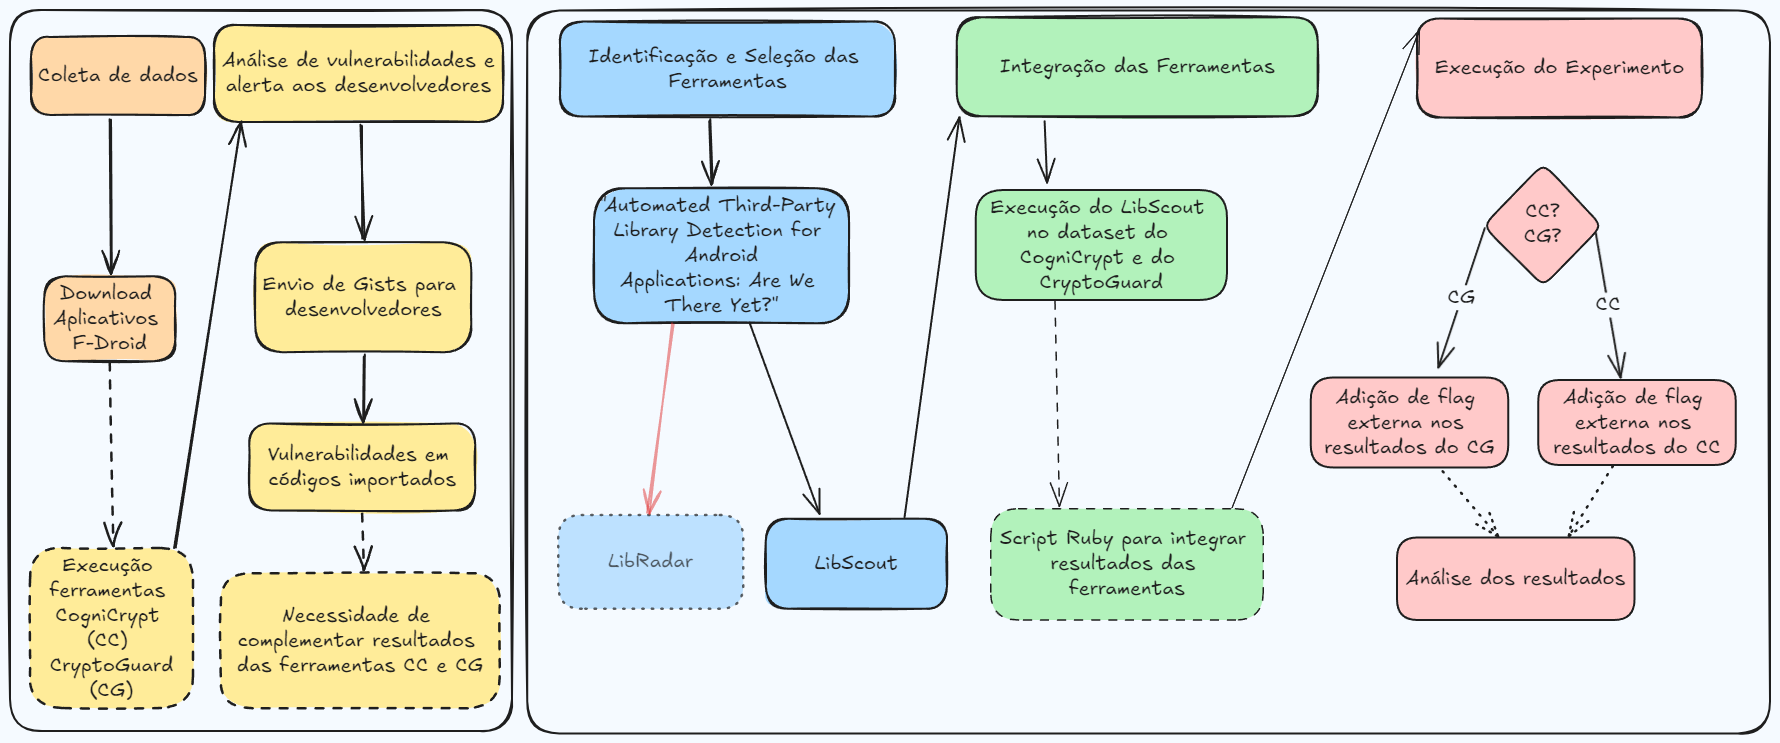
\includegraphics[scale=0.7]{img/research_steps.png}
  \caption{Fases da pesquisa}
  \label{img: research_steps}
\end{figure}